%!TEX root = Physics231.tex

\chapter{Lagrange and Legendre}
\label{ch:Lagrange:Legendre}

Notes on the Legendre transformation as coming from a constrained optimization problem using Lagrange multipliers. Drawing from several sources, but inspired heavily by Tom Witten's Physics 316 (2005) course\footnote{\url{https://jfi.uchicago.edu/~tten/teaching/Physics.316/materials/Legendre.handout.pdf}}. We assume some background in classical mechanics and familiarity with the Legendre transform.

\section{Optimizing a constrained function}

Let $\vec{x} \in \RR^d$ be a point in a $d$-dimensional space and $f(\vec{x})$ be a function. Let $v(\vec{x}) = \bar v$ be a constraint. 
% There may be many constraints, so one may treat $v(\vec{x})$ and $\bar v$ as having multiple components. 
We seek to maximize $f(\vec{x})$ subject to the constraint equation:
\begin{align}
 \max_x \left.f(x)\right|_{v(\vec{x})=\bar v} = f(\bar{\vec{x}})    
 \label{eq:constrained:optimization}
 \ .
\end{align}
Here $\bar{\vec{x}}$ is the point that satisfies the constraint and realizes the [constrained] maximum value of the function $f$.
% 
We may alternatively minimize $f(\vec{x})$ and the discussion below follows identically. If one is really picky, we should say  \emph{supremum} and \emph{infimum} instead of maximum and minimum. 

For the purposes of this document, we assume that $f(x)$ has a single constrained maximum value. Otherwise, one may assume that we focus on a neighborhood around a local maximum so that we may ignore any additional optima or saddle points.


The point $\bar{\vec{x}}$ that realizes the constrained maximum of $f(\vec{x})$ does not satisfy $\nabla f(\bar{\vec{x}}) = 0$. Otherwise $\bar{\vec{x}}$ would be a maximum of the unconstrained function and we could ignore the constraint equation. However, the value of $\nabla f(\bar{\vec{x}})$ must be in the normal direction to the surface of constraint: $\nabla f(\bar{\vec{x}}) \propto \nabla v(\bar{\vec{x}})$.\sidenote{Take a moment to make sure you uderstand why this is true graphically.}

\begin{exercise}
Take a moment to appreciate why $\nabla f(\bar{\vec{x}}) \propto \nabla v(\bar{\vec{x}})$. Consider a two dimensional system $\vec{x}\in \RR^2$ with a constraint equation $$v(\vec{x}) = (x^1)^2 + (x^2)^2 = 1.$$ This forces us to live on the circle $S^1$. \emph{Go ahead and draw this.} Sketch the normal vectors $\nabla v$ on the circle. These are little arrow pointing radially outward.

Now imagine a simple function $f(\vec{x})=x^1$. THe contours of constant $f$ are vertical lines. \emph{Go ahead and add a few contours to your sketch.} You can see that the vector field $\nabla f(\vec{x})$ points in the horizontal direction. 

Observe that $\nabla v \propto \nabla f$ at the points on $S^1$ that extremize $f(\vec{x})$. If this were not the case, then one could imagine moving in the tangential direction---that is, along the constraint surface $S^1$---to increase or decrease the value of $f(\vec{x})$ while satisfying the constraint.
\end{exercise}

\section{Lagrange Multiplier}



The Lagrange multiplier approach to the optimization problem \eqref{eq:constrained:optimization} defines a new function $g(\vec{x})$ that depends on an additional parameter, the Lagrange multiplier $\bar p$:\sidenote{Traditionally the Lagrange multiplier is named something like $\lambda$. We write $\bar p$ deliberately to highlight the duality between position and---\emph{spoilers!}---momentum.}
\begin{align}
    g(\vec{x}) &\defeq f(\vec{x}) - \bar p v(\vec{x}) \ .
\end{align}
The Lagrange multiplier is precisely the proportionality constant between $\nabla f(\bar{\vec{x}})$ and $\nabla v(\bar{\vec{x}})$. This implies that the maximum of the \emph{unconstrained function} $g(\vec{x})$ occurs where $f$ realizes its constrained maximum:
\begin{align}
    \nabla f(\bar{\vec{x}}) &= \bar p \nabla v(\bar{\vec{x}}) 
    % =
    % \frac{d f(\bar{\vec{x}})}{d\bar v}
    &
    \nabla g(\bar{\vec{x}}) &= \nabla f(\bar{\vec{x}}) - \bar p \nabla v(\bar{\vec{x}}) = 0 
    \ .
    \label{eq:unconstrained:maximization}
\end{align}
Finding the maximum of $g(\vec{x})$ thus solves the original problem \eqref{eq:constrained:optimization},
\begin{align}
    \nabla g(\bar{\vec{x}}) &= 0
    &\Rightarrow & &
    \max_x \left.f(x)\right|_{v(\vec{x})=\bar v} = f(\bar{\vec{x}})    \ .
\end{align}


Observe that the expression for $\bar p$ in \eqref{eq:unconstrained:maximization} assumes that one already knows the point $\bar{\vec{x}}$ for which $\nabla g(\bar{\vec{x}})=0$. This appears to lead to a circular argument where our method to solve for $\bar{\vec{x}}$ assumed that we already know $\bar p$. There is a way out. Define an extended function 
\begin{align}
    g(\vec{x};p) \defeq f(\vec{x}) - p v(\vec{x}) \ .
    \label{eq:Lagrange:g:as:free:energy}
\end{align}
where $p$ is a free parameter. The gradient $\nabla$ is assumed to only act on the $\vec{x}$ directions so that $\nabla g(\vec{x};p) =0$ yields $\bar{\vec{x}}$ as a function of the free parameter $p$, $\bar{\vec{x}}(p)$.

We find the `correct' value $p=\bar p$ by plugging the function $\bar{\vec{x}}(p)$ into the constraint equation
\begin{align}
    \left.v(\bar{\vec{x}}(p))\right|_{p=\bar p} &= \bar v \ .
\end{align}

\begin{example}\label{eg:circle:line}
Consider $\vec{x} = (x,y)^{\trans} \in \RR^2$ and the function $f(\vec{x}) = x^2 + y^2$ subject to the constraint $v(\vec{x}) = ax + by = \bar v$. We parameterize the constrained subspace by $(x, y(x))^{\trans}$ where
\begin{align}
    y(x) &= \bar v - \frac{a}{b}x \ .
\end{align}
The unconstrained maximization condition $\nabla g(\vec{x};p) = 0$ gives
\begin{align}
    \partial_x g(\vec{x};p) = 2x - pa &=0
    &
    \partial_y g(\vec{x};p) = 2y - pb &=0 \ .
\end{align}
We find that as a function of the Lagrange multiplier, $p$, the maximum is attained at
\begin{align}
    \bar{\vec{x}}(p) =
    \frac{p}{2}
    \begin{pmatrix}
        a\\
        b
    \end{pmatrix}
    \label{eq:eg:simple:multiplier:xp}
    \ .
\end{align}
The correct value of the Lagrange multiplier is $p=\bar p$ where
\begin{align}
    v(\bar{\vec{x}}(\bar p)) =  
    % \left(\frac{a^2}{2} + \frac{b^2}{2}\right)  
    \frac{1}{2}(a^2 + b^2)\bar p
    = \bar v \ .
    \label{eq:eg:simple:multiplier:solve:p}
\end{align}
For concreteness, consider the case $a = b = \bar v = 1$. Then \eqref{eq:eg:simple:multiplier:solve:p} gives $\bar p = 1$. Equation~\eqref{eq:eg:simple:multiplier:solve:p} tells us that $\bar p = 1$. Then we find that \eqref{eq:eg:simple:multiplier:xp} indeed gives us that $f(\vec{x})$ attains its constrained maximum at $\bar{\vec{x}} = \tfrac{1}{2}(1, \, 1)^{\trans}$. 
\end{example}

\section{Looking familiar?}

In classical mechanics, the constraint function $v(\vec{x})$ is the velocity. The form of the constraint forces the $v(\vec{x})$ to be the time derivative of the trajectory. The Lagrange multiplier $\bar p$ is indeed the momentum, the conjugate variable to the velocity. 

\section{A symmetric formulation}

Our expressions are nicer if we replace $g(x)$ by its negative value. We thus define
\begin{align}
    h(\vec{x}) &\defeq - g(\vec{x}) = \bar p v(\vec{x}) - f(\vec{x}) \ .
\end{align}
Here $p$ and $\bar p$ are the same as above. Since we maximize $f(x)$, we must \emph{minimize} $h(x)$. The corresponding extended function is
\begin{align}
    h(\vec{x}; p) &\defeq - g(\vec{x};p) = p v(\vec{x}) - f(\vec{x}) \ .
    \label{eq:h:x:p}
\end{align}
The Lagrange multiplier procedure follows identically as in the case for $g(\vec{x};p)$. We work with $h(\vec{x})$ and $h(\vec{x};p)$ in what follows. You may alternatively read $-g$ everywhere. The reason for the the function $h(\vec{x})$ is that we may write at the optimum value $\bar{\vec{x}}$ in a symmetric way:
\begin{align}
    f(\bar{\vec{x}}) + h(\bar{\vec{x}}) = \bar p \bar v \ .
    \label{eq:pre:Legendre:f:h:p:v}
\end{align}
This will aid in our transition to identifying $f$ and $h$ as Legendre transforms of one another with $\bar p$ and $\bar v$ as conjugate variables. One could also choose the alternate sign convention where $f$ and $g$ are Legendre transformations of one another.





\section{Lagrange Multiplier as a Function}

The Lagrange multiplier $\bar p$ is the proportionality between two gradients at $\bar{\vec{x}}$. One can see this from \eqref{eq:unconstrained:maximization}. It is suggestive to write the formally nonsensical expression\sidenote{Do you see why this is nonsense? $\bar p$ is a scalar quantity. The right-hand side is a ratio of vectors. What does it mean to divide two vectors? If you bring up geometric algebra here, I'm going to plug my fingers into my ears and pretend that I can't hear you.}
\begin{align}
    \bar p &= \left.\frac{\nabla f(\vec{x})}{\nabla v(\vec{x})}\right|_{\vec{x}=\bar{\vec{x}}} \ ,
\end{align}
where the ratio of two vectors is \emph{only} makes sense here because $\nabla f(\bar{\vec{x}}) \propto \nabla v(\bar{\vec{x}})$. To make this more sensible, we recall that $\nabla v(\vec{x})$ points in the direction of increasing level surfaces. In other words, it is the direction in $\RR^d$ corresponding to $v(\vec{x}) = \bar v + \delta \bar v$ with $\delta \bar v >0$. This motivates an extended version of $f(\vec{x})$:
\begin{align}
    f(\vec{x};\bar v) \defeq
    \left. f(\vec{x}) \right|_{v(\vec{x}) = \bar v} \ .
\end{align}
We say `extended' because $f$ now has an additional argument---but really this is the \emph{constrained} function $f(\vec{x})$ whose domain is the solution to the constraint equation $v(\vec{x}) = \bar v$. This means that we may write the Lagrange multiplier $\bar p$ as a derivative with respect to $\bar v$ on this extended function:
\begin{align}
    \bar p &= 
    \left.\frac{\D f(\vec{x}; v)}{\D v}\right|_{\vec{x}=\bar{\vec{x}}, \, v = \bar v} 
    \ .
    \label{eq:bar:p:differential}
\end{align}
The $v$ in this expression is a variable that is set to $\bar v$. It is \emph{not} the function $v(\vec{x})$. 

We may generalize the expression for the Lagrange multiplier \eqref{eq:bar:p:differential} in light of a desire to cast this problem on a dual footing. In \eqref{eq:pre:Legendre:f:h:p:v}, $\bar p$ and $\bar v$ are conjugate variables, where the $\bar v$ is understood to specify the level curve of some constraint function $v(\vec{x})$. We may imagine $\bar p$ to be the analogous object defined extending \eqref{eq:bar:p:differential}:
\begin{align}
    p(\vec{x}) &\defeq
    \left.\frac{\D f(\vec{x}; v)}{\D v}\right|_{v = \bar v} 
    \ .
    \label{eq:p:differential:function}
\end{align}
We now have the ingredients to anticipate a dual formulation of the optimization problem where we seek to minimize $h(\vec{x})$ subject to a constraint $p(\vec{x}) = \bar p$.


% \begin{example}
% The expression \eqref{eq:p:differential:function} for $p(\vec{x})$ is  the inverse of the solution $\bar{\vec{x}}(p)$ to $\nabla h(\bar{\vec{x}}(p);p) = 0$. We may check this explicitly:
% \begin{align}
%     \nabla h(\vec{x};p) = p \nabla v(\vec{x}) - \nabla f(\vec{x}) = 0 \ .
% \end{align}
% \end{example}

\section{Dual constraint equation}
One would also like the dual formulation of \eqref{eq:p:differential:function}:
\begin{align}
    v(\vec{x}) &\equiv 
    \left.\frac{\D h(\vec{x}; p)}{\D p}\right|_{p = \bar p} 
    &
    \bar v & = 
    \left.\frac{\D h(\vec{x}; p)}{\D p}\right|_{\vec{x}=\bar{\vec{x}}, \, p = \bar p} 
    \ .
    \label{eq:v:differential:function}
\end{align}
This is an opportunity for a consistency check since the constraint function $v(\vec{x})$ is assumed to have been part of the statement of the original problem. We see that from the definition of $h(\vec{x};p)$ in \eqref{eq:h:x:p}, 
\begin{align}
    \left. \frac{ \D h( \vec{x}; p ) }{ \D p } \right|_{p = \bar p} 
    &= 
    \frac{ \D{} }{ \D{} p }
    \left(
        pv(\vec{x}) - f(\vec{x})
    \right)_{p = \bar p} 
    =
    v(\vec{x}) \ .
\end{align}
The identification of $v(\vec{x})$ as a derivative of $h(\vec{x};p)$ is thus consistent and nicely parallels the functional expression \eqref{eq:p:differential:function}.  

\section{Legendre Transform}

Let us define the functions at their constrained extrema:
\begin{align}
    \bar f(\bar v) 
        &
        \defeq f(\bar{\vec{x}}, \bar v)
        = \max_\vec{x} f(\vec{x}, \bar v)
    &
    \bar h(\bar p) 
        &
        \defeq h(\bar{\vec{x}}, \bar p) 
        = \min_\vec{x} h(\vec{x}, \bar p)
        \ .
\end{align}
We say that $\bar f(\bar v)$ and $\bar h(\bar p)$ are \textbf{Legendre transformations} of one another with \textbf{conjugate variables} $\bar v$ and $\bar p$. The symmetric expression \eqref{eq:pre:Legendre:f:h:p:v} can now be written with the `natural' conjugate variables manifest: 
\begin{align}
    \bar f(\bar v) + \bar h (\bar p)  = \bar p \bar v \ .
\end{align}
The bars on these expressions are now cumbersome and reflect the origin of these expressions from an optimization problem over a variable, $\vec{x}$, which has fallen by the wayside. To be clear: in the original optimization problem, our goal was to find $\bar{\vec{x}}$ that optimized $f(\vec{x})$. Our goal has now shifted to understanding the dual structure of the Legendre transformation. 
% 
At this point, we may drop the bars on the conjugate variables $\bar p \to p$ and $\bar v \to v$. However, we shall keep the bars on $\bar f$ and $\bar h$ to avoid confusing them with the original functions $f(\vec{x})$ and $h(\vec{x})$ in the optimization problem.

The Legendre pair is thus
\begin{align}
    \bar f(v) + \bar h (p)  =  p v \ ,
    \label{eq:Legendre:eq}
\end{align}
with the identification that $p$ and $v$ are derivatives:
\begin{align}
    p &= \frac{\D{\bar f}(v)}{\D v}
    &
    v &= \frac{\D{\bar h}(p)}{\D p} \ .
    \label{eq:Legendre:eq:derivatives}
\end{align}

\begin{example}
We confirm the conjugate relations \eqref{eq:Legendre:eq:derivatives}:
\begin{align}
    \frac{\D{\bar f}(v)}{\D v} &=
    \frac{\D{}}{\D{v}}\left(pv - \bar h(p)\right)
    =
    p + v\frac{\D{p}}{\D{v}} 
    - \frac{\D{\bar h}}{\D{p}}
      \frac{\D{p}}{\D{v}}
    = p \ ,
\end{align}
where we use $v= \bar h'(p)$. Similarly
\begin{align}
    \frac{\D{\bar h}(p)}{\D p} &=
    \frac{\D{}}{\D{p}}\left(pv - \bar f(v)\right)
    =
    v + p\frac{\D{v}}{\D{p}} 
    - \frac{\D{\bar f}}{\D{v}}
      \frac{\D{v}}{\D{p}}
    = v \ ,
\end{align}
where we use $p= \bar f'(v)$. 
\end{example}

\section{Graphical interpretation}

The Legendre transformation is usually not defined with respect to an optimization problem. Indeed, \eqref{eq:Legendre:eq} does not refer to any optimization over $\bar{\vec{x}}$ at all. The function $\bar f(v)$ is a function of the variable $v$ that, a priori, has nothing to do with $\vec{x}$. Recall that $v$ (n\'ee $\bar v$) defined a level curve of the constraint equation.


\begin{figure}[tb]
    \centering
    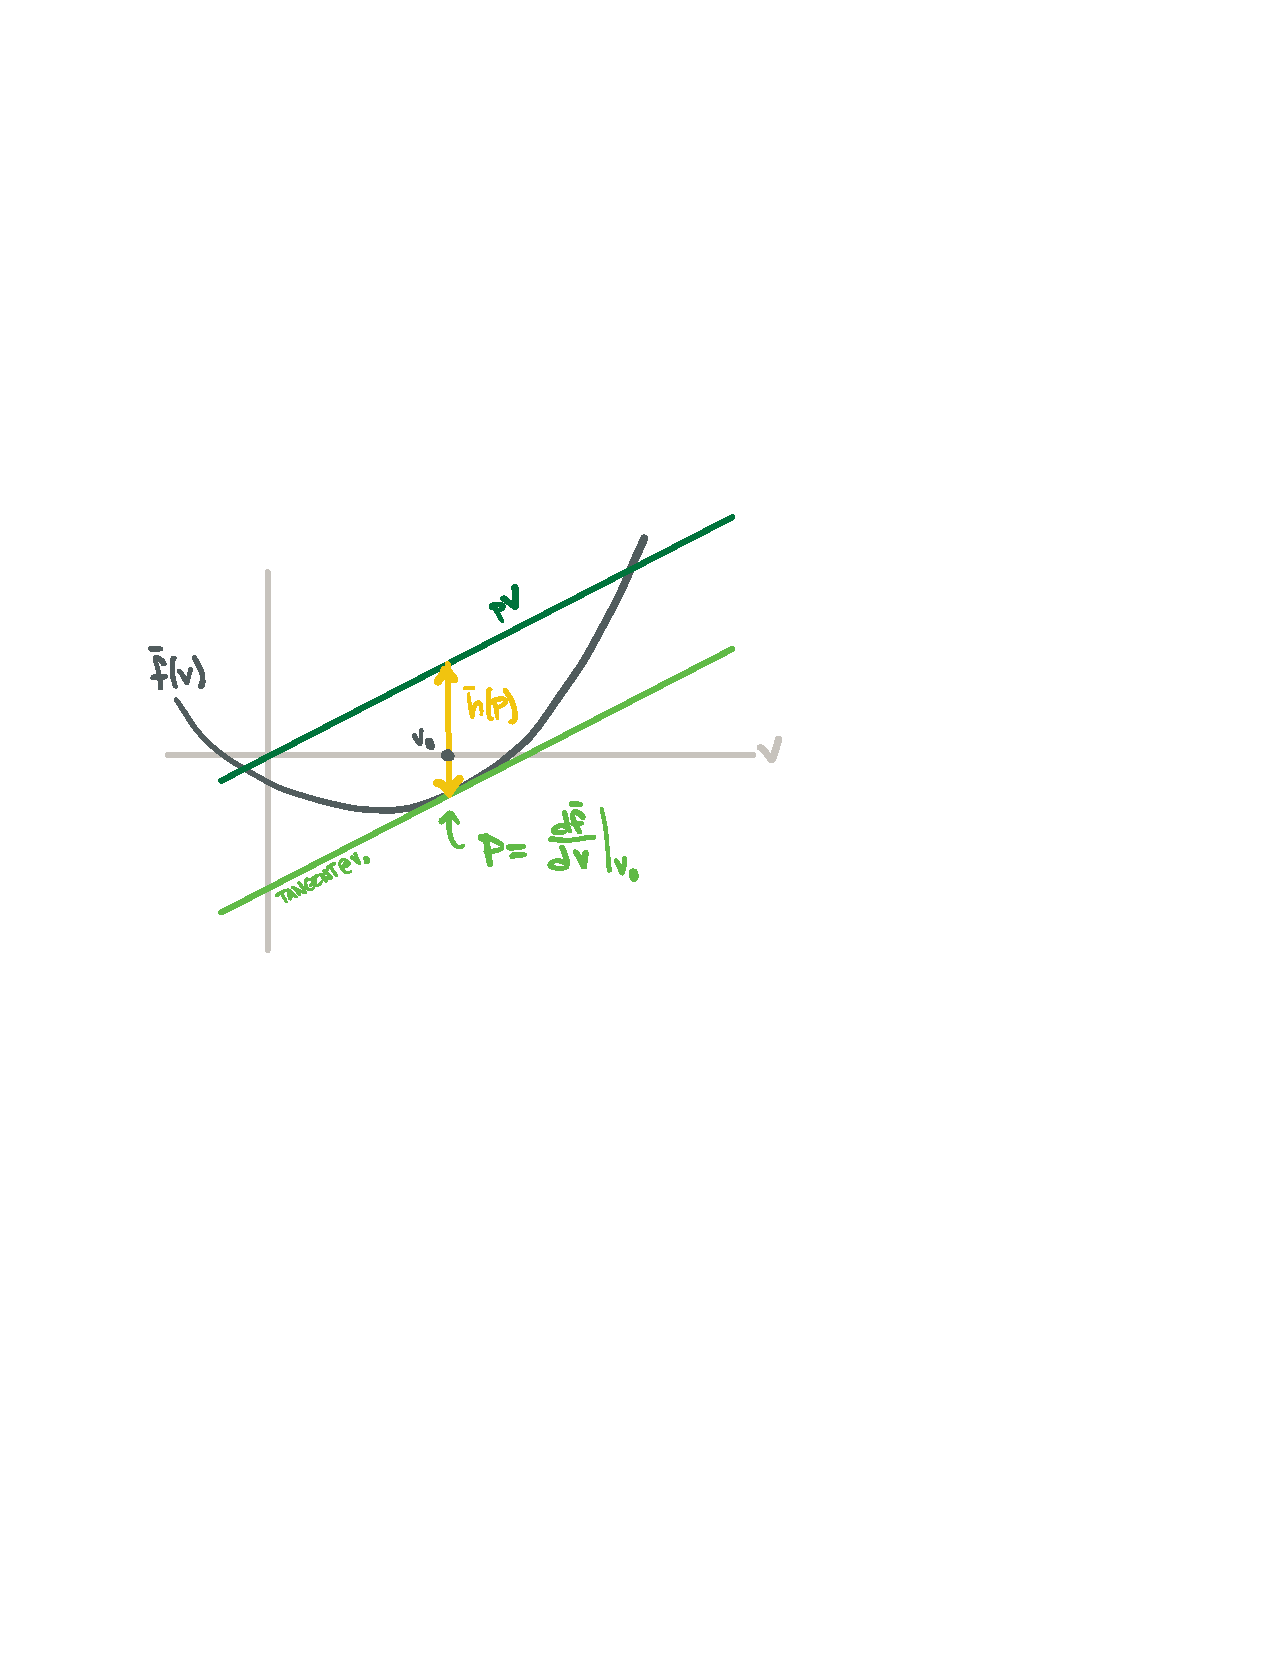
\includegraphics[width=0.5\linewidth]{figures/Legendre.pdf}
    \caption{Legendre transform, graphically. The Legendre transformation $\bar h(p)$ is the difference between $pv_0$ and $f(v_0$) where $v_0$ is the point where $f'(v_0)=p$. }
    \label{fig:Legendre:fig}
\end{figure}


Fig.~\ref{fig:Legendre:fig} is a graphical representation of the Legendre transformation.\sidenote{Much to my horror Fig.~\ref{fig:Legendre:fig} shows $\bar f(v)$ as having a minimum. In the text I have implied that $\bar f(v)$ has a maximum. This does not affect the conclusions. Good luck getting me to redraw that figure.} We assume that $\bar f$ is \textbf{convex}. This means that we are in the neighborhood of a local minimum so that there is a one-to-one mapping between first derivatives $\bar f'$ and points $v$. We identify the Legendre transformation of $\bar f$ at $v_0$ with $\bar h(p)$, where $p$ is the slope of $\bar f(v_0)$. $\bar h(p)$ is the offset between the line $y=pv$ and $f(v)$ at $v_0$. We see that this matches the definition \eqref{eq:Legendre:eq} with appropriate choice of the sign of the difference.

\section{Legendre as an Optimization Problem}

An equivalent definition of the Legendre transformation is
\begin{align}
    \bar h(p) \defeq \max_{v}\left[pv-\bar f(v)\right] \ .
\end{align}
This optimization has nothing to do with the optimization over $\vec{x}$ in our Lagrange multiplier problem.
% 
This is illustrated in Fig.~\ref{fig:Legendre:3D}. It represents an optimization over an extended function, 
\begin{align}
 \bar h(p,v) = pv - \bar f(v) \ .   
\end{align}
Note that this extended function should not be confused with the extended function $h(\vec{x};p)$ in \eqref{eq:h:x:p}. The extended function $\bar h(p,v)$ is formally a function of both $p$ and $v$. 
% 
Unlike the definition in \eqref{eq:Legendre:eq}, the variables $p$ and $v$ are unrelated to each other. 
% 
The Legendre transform $\bar h(p)$ of $\bar f(v)$ is the maximum of $\bar h(p,v)$ over $v$ for a fixed value of $p$.
% 
We can see from the graphical representation in Fig.~\ref{fig:Legendre:fig} that these definitions are equivalent for convex functions:
\begin{align}
    \bar h(p) =
    % \max_{v}\left[pv-\bar f(v)\right]
    \max_{v} \bar h(p,v)
    &=
    \left[pv-f(v)\right]_{p=\bar f'(v)} \ .
\end{align}
The left-hand side seems to be the standard definition in mathematics\sidenote{with maximum replaced with supremum, of course}, while the right-hand side is the form invoked in physics. The condition that $p=\bar f'(v)$ is understood to be a restriction on $v$. The definition with a supremum is more general and does not assume a differentiable, convex function---it is called the Legendre--Fenchel transformation.
% https://www.ise.ncsu.edu/fuzzy-neural/wp-content/uploads/sites/9/2019/01/or706-LF-transform-1.pdf

\begin{figure}[tb]
    \centering
    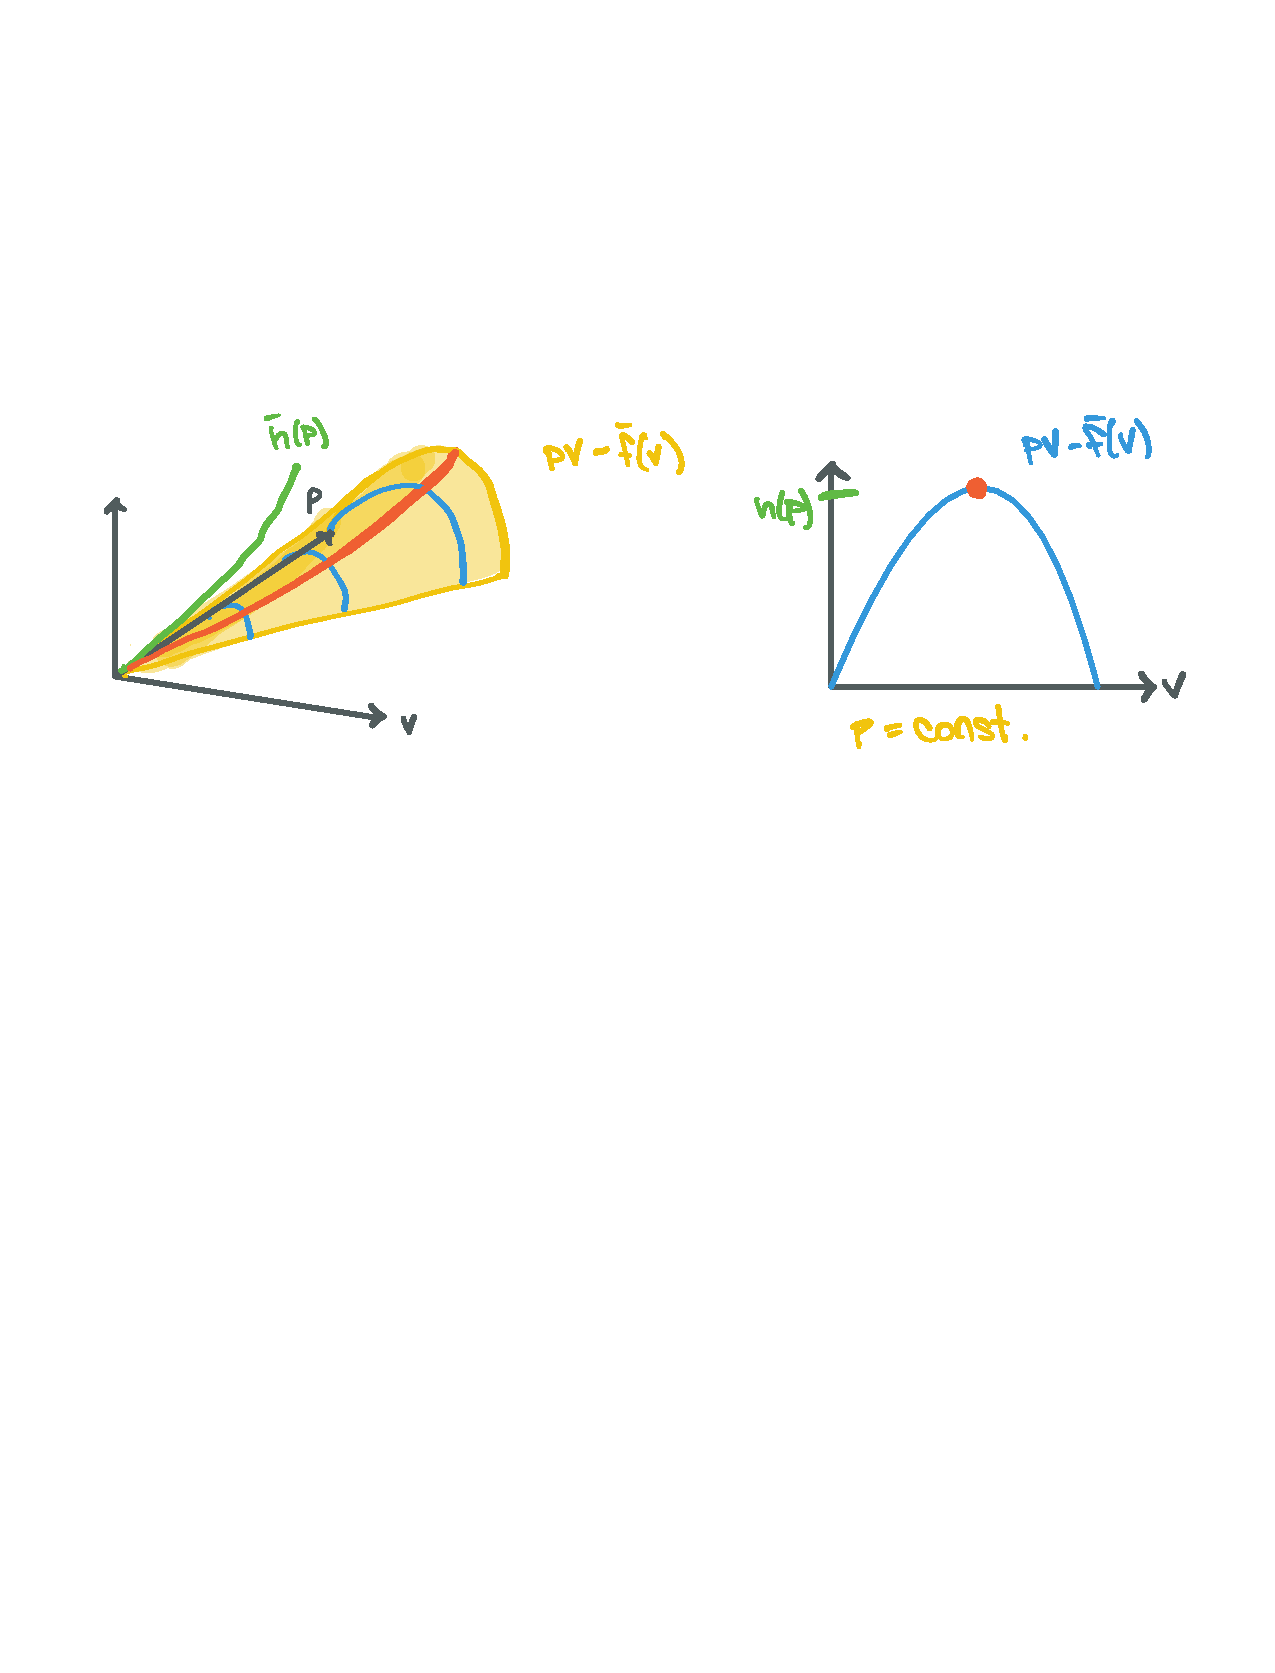
\includegraphics[width=\linewidth]{figures/Legendre3D.pdf}
    \caption{Illustration of the Legendre transformation as the supremum of the extended functions. Adapted from Mark Alford's {WUSTL} lecture notes (2019).}
    \label{fig:Legendre:3D}
\end{figure}

\section{Legendre from Derivatives}

Alternatively, we may take the conjugate variables \eqref{eq:Legendre:eq:derivatives} as a starting point for defining the Legendre transformation. Let us define the anti-derivatives\sidenote{By this I mean an indefinite integral.} of the functions $\bar f$ and $\bar h$
\begin{align}
    F(p) &\defeq 
    \left(\frac{\D{\bar f}}{\D{v}}\right)^{-1}
    &
    H(v) &\defeq 
    \left(\frac{\D{\bar h}}{\D{p}}\right)^{-1}
    \ .
\end{align}
The overall constant is chosen so that $F(p) = v$, where $\bar f'(v)= p$. Similarly, $H(v)=p$ where $\bar h'(p) = v$. Note that the choice of variables here matches \eqref{eq:Legendre:eq:derivatives}. 

Let us define the functions
\begin{align}
    \tilde h(v) &\defeq p v - f(v)
    &
    \tilde f(p) &\defeq p v - h(p) \ .
\end{align}
While $\tilde h(v)$ and $\bar h(p)$ have the same form, we understand the former to be a function of $v$ while the latter is a function of $p$.  % Analogously, the expressions $p(v)$ and $v(p)$ are understood in the sense of \eqref{eq:Legendre:eq:derivatives}.  
% 
The definitions of the anti-derivatives mean that $F(p)$ is the critical point of $\tilde h(v)$:
\begin{align}
    \left.\tilde h'(v)\right|_{v=F(p)} = p - \left.f'(v)\right|_{v=F(p)} = 0 \ .
\end{align}
At the point $v=F(p)$,
\begin{align}
    \bar h(p) &= p F(p) - \bar f(F(p))
    &
    \bar h'(p) &= F(p) + p F'(p) 
    - \left.\frac{\D{\bar f}}{\D{v}}\right|_{v=F(p)}
        % \frac{\D{ F(p)}}{\D{p}}
        F'(p) \ .
\end{align}
On the right-hand side we impose defining equation \eqref{eq:Legendre:eq:derivatives} where $p\equiv \D{\bar f}/\D{v}$ evaluated at $v=F(p)$. This gives
\begin{align}
    \bar h'(p) = F(p) = \left(\bar f'(v)\right)^{-1} \ .
\end{align}
By the same argument,
\begin{align}
    \bar f'(v) = H(v) = \left(\bar h'(p)\right)^{-1} \ .
\end{align}
We see that the derivatives of the Legendre transformation are the inverse of the derivative of a function.



\subsection{Legendre as an Involution}

An \textbf{involution} is a transformation that is its own inverse. Applying an involution twice returns one to the original state. The Legendre transformation is an involution, though this is not obvious from the graphical representation. The first hint of this is the symmetric expression \eqref{eq:Legendre:eq} where the pairs $\{\bar f, v\}$ and $\{\bar h, p\}$ are on equal footing. This means that if $\bar f$ is the Legendre transformation of $\bar h$, then it must be true that $\bar h$ is the Legendre transformation of $\bar f$. 

\begin{figure}[tb]
    \centering
    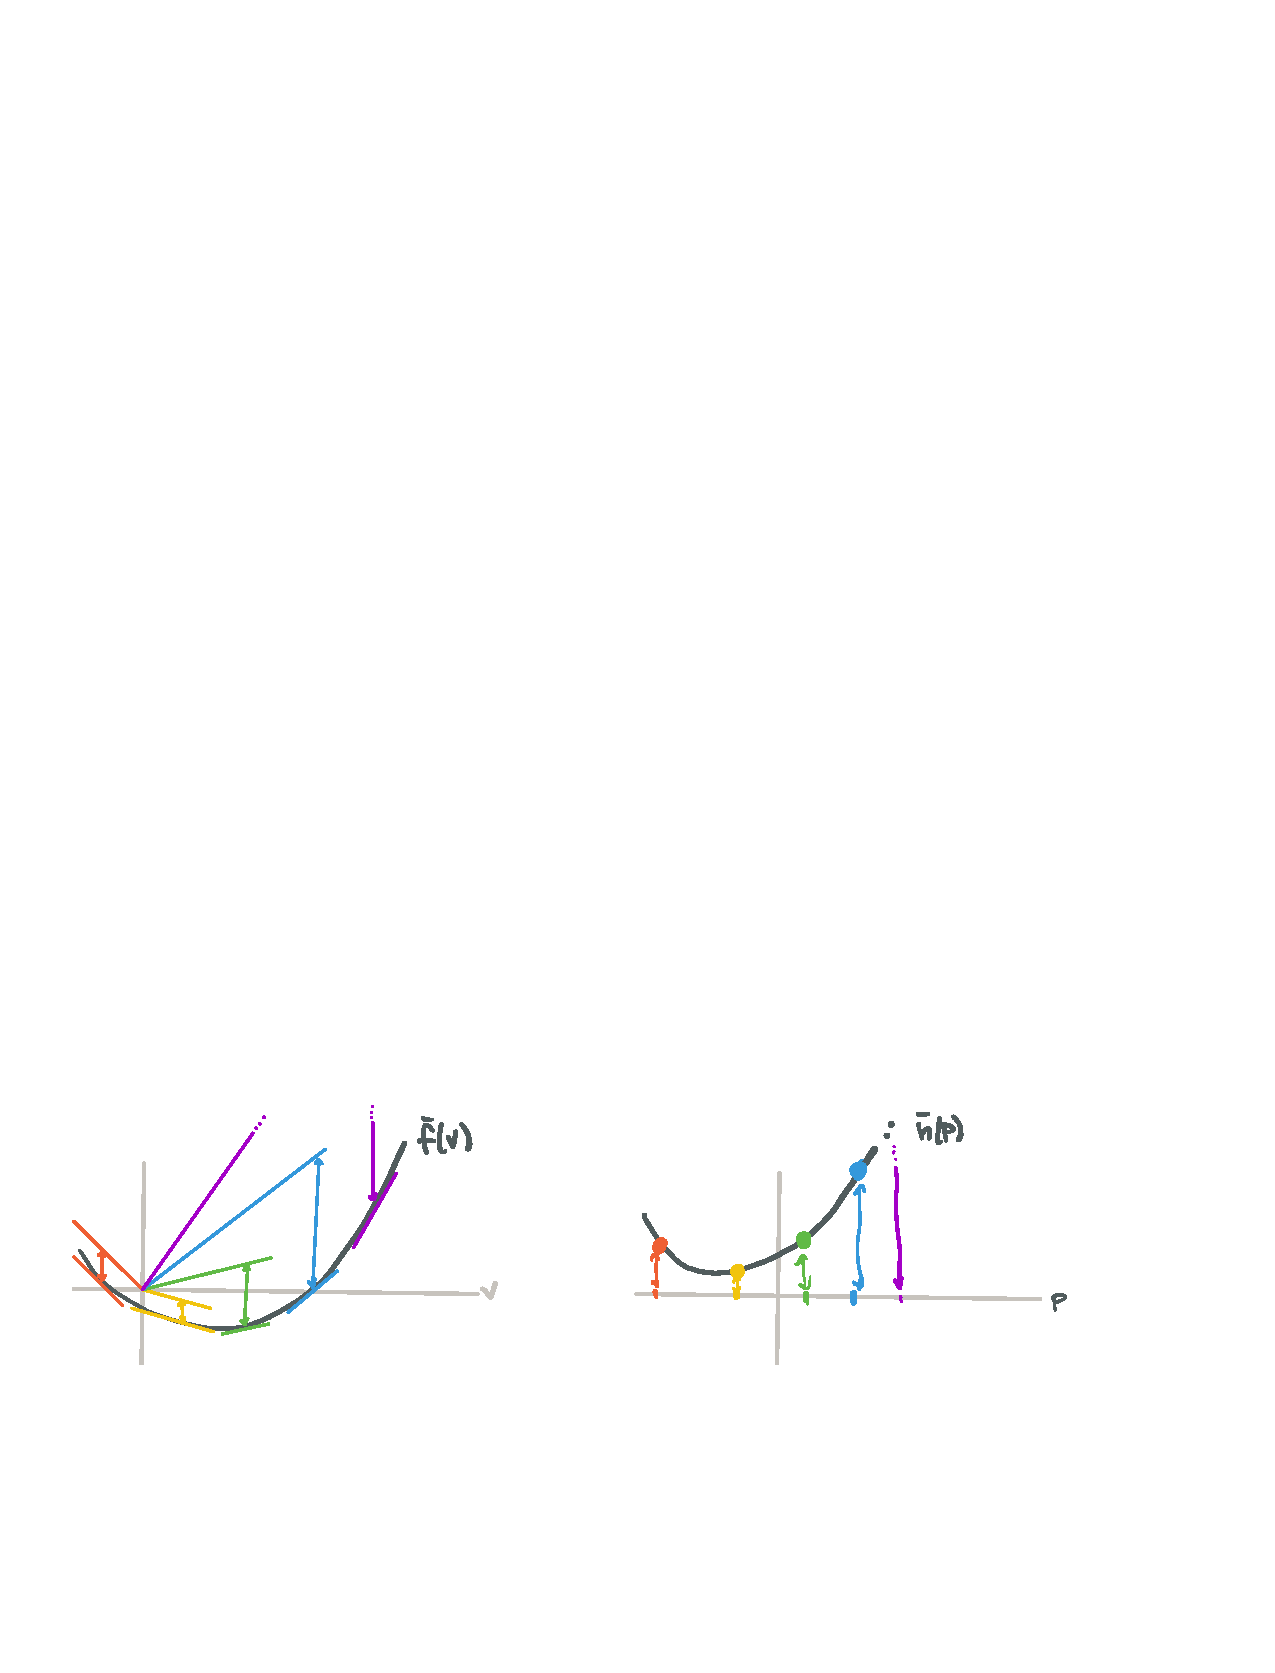
\includegraphics[width=\linewidth]{figures/LegendreLegendre.pdf}
    \caption{Left: $\bar f(v)$ is a function. For different colored points, the arrows indicate $vp-\bar f(v)$. Right: the Legendre transform $\bar h(p)$ where different values of $p$ correspond to the slopes of $\bar f(v)$ and $\bar h(p)$ shows the corresponding length of the arrows from the $\bar f(v)$ plot on the left.}
    \label{fig:Legendre:plot}
\end{figure}

Another view of this from Harald Skarke\footnote{\url{https://arxiv.org/abs/1209.6193}} makes the dual nature of $\bar h(p)$ and $\bar f(v)$ more manifest using the relation between derivatives of Legendre pair functions above:
\begin{align}
    p &= \frac{ \D{\bar f}(v) }{ \D{v} }
    &
    v &= \frac{ \D{\bar h}(p) }{ \D{p} }
    \label{eq:p:v:as:derivatives}
    \ .
\end{align}
The fact that $\bar f'(v)$ and $\bar h'(p)$ are inverses tells us that we can understand these as the slopes of the \emph{same line} in the $v$--$p$ plane taken with respect to each axis. We illustrate this in Fig.~\ref{fig:Legendre:area}.

\begin{figure}[tb]
    \centering
    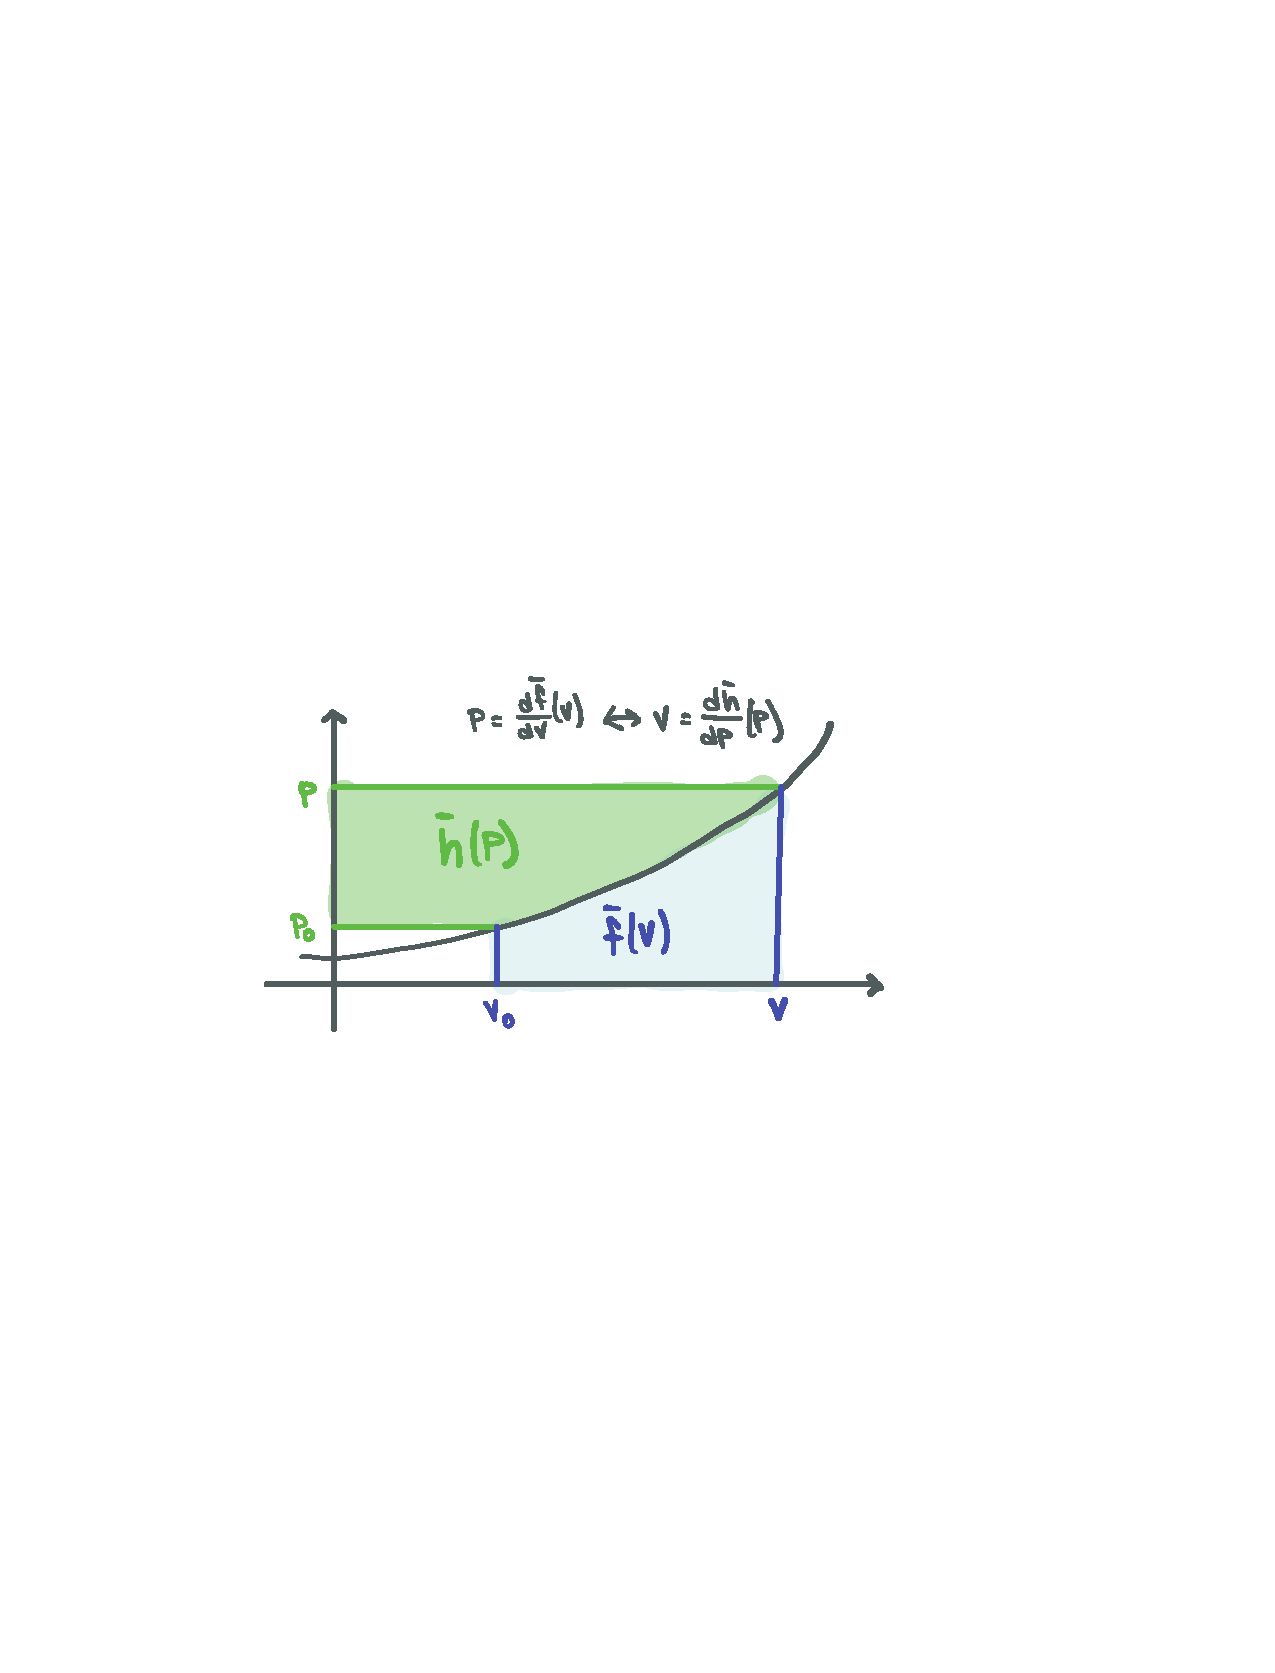
\includegraphics[width=.7\linewidth]{figures/LegendreArea.pdf}
    \caption{Illustration of the involutive nature of the Legendre transformation adapted from Skarke, \texttt{arXiv:1209.6193}. }
    \label{fig:Legendre:area}
\end{figure}

The Legendre transformation pair of functions $\bar f(v)$ and $\bar h{p}$ are integrals of their respective derivatives \eqref{eq:p:v:as:derivatives}. In Fig.~\ref{fig:Legendre:area} this is the area `under the curve' relative to the two different axes, 
\begin{align}
    \bar f(v) &= \int^v_{v_0} \D{v}\, p(v)
    &
    \bar h(p) &= \int^p_{p_0} \D{p}\, v(p) \ .
\end{align}
These are defined with respect to an arbitrary reference point $(v_0, p_0)$ on the curve. This means that our expressions for $\bar f(v)$ and $\bar h(p)$ are defined up to an overall constant. 

We remark that Fig.~\ref{fig:Legendre:area} assumes that the function $p(v)$---or equivalently $v(p)$ is monotonically increasing. For our purposes, this is sufficient to illustrate the duality of the Legendre transform. We refer to \texttt{arXiv:1209.6193} for further discussions.

\section{Additional Variables}

Suppose $\bar f$ depends on other variables in addition to $v$, 
\begin{align}
    \bar f = \bar f(q,v) \ .
\end{align}
We treat $q$ as an auxiliary variable: we do not perform a Legendre transformation with respect to it. This implies that the Legendre transform $\bar h$ also depends on the additional variable $q$, $\bar h = \bar h(q,p)$. In classical mechanics, position is an auxiliary variable of this type. Partial derivatives with respect to the auxiliary variable are equal:
\begin{align}
    \left.\frac{\partial \bar h(q,p)}{\partial q}\right|_{p}
    =
    \frac{\partial}{\partial q}\left(pv - \bar f(q,v)\right)_{p}
    =
    p\frac{\partial v}{\partial q}
    -
    \frac{\partial \bar f}{\partial v}
    \frac{\partial v}{\partial q}
    -
    \frac{\partial \bar f}{\partial q}
    =
    -\frac{\partial \bar f}{\partial q} \ .
    \label{eq:auxiliary:variable:derivatives}
\end{align}
We have used the fact that the partial derivative of $\bar h(q,p)$ with respect to $q$ holds $p$ fixed, but we must allow $v$ to potentially depend on $q$. The minus sign is somewhat annoying, so here it is useful to use $\bar g(q,p) \equiv -\bar h(q,p)$ as the Legendre pair so that
\begin{align}
    \frac{\partial \bar f}{\partial q}
    = 
    \frac{\partial \bar g}{\partial q} \ ,
\end{align}
where it is understood that on the left-hand side we hold $v$ fixed while on the right-hand side we hold $p$ fixed.


\section{Multiple Constraints}

In our discussion so far, we started with a single constraint equation $v(\vec{x})=\bar v$ which we imposed with a Lagrange multiplier $p$. We then worked to promote $p$ into a bona fide dual variable. If there are multiple constraints,
\begin{align}
    v_i(\vec{x}) = \bar v_i \ ,
\end{align}
we would then introduce multiple Lagrange multipliers $p_i$ such that
\begin{align}
    g(x;p_i) &\defeq f(x) -  \sum_i p_i v_i(\vec{x}) 
    &
    h(x;p_i) = -g(x;p_i)
    \ .
\end{align}
The analysis above follows for each conjugate variable pair $(v_i, p_i)$. We write the extended Legendre transform
\begin{align}
     \bar h(p_i, v_i) = \sum_i p_i v_i - \bar f(v_i) \ ,
 \end{align}
 where we understand that $\bar h(p_i)$ is the maximum over $v_i$ or alternatively the identification that $v_i$ satisfies $p_i = \partial_{v_i} \bar f(v_j)$. 
 In the continuum (field theory) limit, 
 \begin{align}
     i&\to y
     &
     v_i &\to v(y)
     &
     p_i &\to p(y) \ .
 \end{align}
 This gives the Legendre transformation of $\bar f(v)$ with $v=v(y)$,
 \begin{align}
     \bar h(p, v) = \int \D{y} \, \left[p(y) v(y) - \bar f(v(y))\right] \ .
 \end{align}


\section{Application: Classical Mechanics, basic form}

We seek to minimize the Lagrangian $\mathcal L[q,\dot q]$ where $q$ is an auxiliary variable. For simplicity on a first pass, we assume no relation between $\dot q$ and $q$. The Legendre transform of $\{\mathcal L, \dot q\}$ is $\{\mathcal H, p\}$. This means that
\begin{align}
    \mathcal L[q,\dot q] &= p\dot q - \mathcal H[q,p]
    &
    \mathcal H[q,p] &= p\dot q - \mathcal L[q,\dot q] \ .
\end{align}
Here $\mathcal L$ and $\mathcal H$ are what we called $\bar f$ and $\bar h$ above. The conjugate variables satisfy
\begin{align}
    \dot q &= \frac{\partial \mathcal H}{\partial p}
    &
    p &= \frac{\partial \mathcal L}{\partial \dot q} \ .
    \label{eq:Lagrangian:basic:p:q}
\end{align}
We may write extended functions where the constraints \eqref{eq:Lagrangian:basic:p:q} are not imposed. 
\begin{align}
    \mathcal L[q,\dot q, p] &= p\dot q - \mathcal H[q,p]
    &
    \mathcal H[q,p, \dot q] &= p\dot q - \mathcal L[q,\dot q] 
    \ ,
\end{align}
where we understand $p$ and $\dot q$ to be independent. The Hamiltonian is understood to be
\begin{align}
    \mathcal H[q,p] &= \max_{\dot q} \mathcal H[q,p,\dot q] \ ,
\end{align}
which imposes a relationship $\dot q(p)$. In this way, $\mathcal H[q,p]$ is purely a function of $p$ via
\begin{align}
    \mathcal H[q,p]
    =
    \mathcal H[q,p,\dot q(p)] \ .
\end{align}





\section{Application: Classical Mechanics, carefully}

The classical trajectory of a point particle, $q(t)$, is the one that minimizes the action,
\begin{align}
    S[q] = \int \D{t}\, \mathcal L(q,\dot q, t) \ .
\end{align}
As a functional, the Lagrangian takes $\dot q(t)$ as an independent argument from $q(t)$. However, we know that $\dot q(t) = \D{q}(t)/\D{t}$ is the time derivative of the trajectory and is \emph{not} independent. This is thus a constrained optimization problem. We thus introduce $v(t)$, an independent velocity, and set $\dot q(t) = v(t)$ using a Lagrange multiplier field $p(t)$. We write the unconstrained field---the analog of $g(x)$---as
\begin{align}
    \tilde S[q,v] &\defeq
    S[q] - \int \D{t}\, p(t)\left[v(t)-\dot q(t)\right] \ ,
\end{align}
where we understand $\dot q(t) = \D{q}/\D{t}$. 
% 
The term in brackets that multiplies the Lagrange multiplier $p(t)$ is the analog of $v(\vec{x})$ in the simpler problem above.\footnote{The nomenclature here is unfortunately a bit confusing when comparing our formalism above to the steps here.}
% 
$q(t)$ is an auxiliary variable in this problem.
% 
The Legendre conjugate variables are $\dot q$ and $p$. Following the discussion of multiple constraints in the continuum limit, it is more precise to say that $\dot q(t)$ and $p(t)$ are conjugate variables for each continuous value of $t$.

The variation of the unconstrained $\tilde S$---the analog of the variation of $g(\vec{x})$---contains variations in the position $q(t)$ and the constrained field $v(t)$ that is to be identified with the velocity $\dot q(t)$. Since we are focused on the Legendre transformation, one may think that the variation with respect to $q(t)$ is not significant for our study. However, the $q(t)$ variation will be the object of an important integration by parts:
\begin{align}
    \delta \tilde{S}[q,v]
    &= \int \D{t}
    \left[
        \frac{\delta \mathcal L}{\delta q} 
        - 
        \frac{\D{p}(t)}{\D{t}}
    \right] \delta q(t)
    +
    \int \D{t}
    \left[
        \frac{\delta \mathcal L}{\delta v} 
        - 
        p(t)
    \right] \delta v(t) \ .
\end{align}
As per the usual convention, we write functional derivatives as $\delta/\delta f(t)$. This essentially $\partial/\partial{f_i}$ in the $f_i\to f(t)$ continuum limit.
In order for $\delta \tilde S = 0$, each of the brackets must vanish. This gives the expressions
\begin{align}
    \frac{\delta \mathcal L}{\delta q} 
    &= \dot p(t)
    &
    \frac{\delta \mathcal L}{\delta v}
    &= p(t) 
    \ . 
    \label{eq:classical:mechanics:dLdv:p}
\end{align}
The first expression is simply the condition from varying with respect to $\delta q(t)$. The second expression is an implicit expression for how $v$ depends on $p$, that is $v(t)=v[p(t)]$. This step is analogous to \eqref{eq:Legendre:eq:derivatives}. If one solves for $p(t)$, one recovers the Euler--Lagrange equation of motion wherein $v(t) = \dot q(t)$. To proceed analogously with the Legendre transformation, we instead replace $v(t)$ with $p(t)$ using the right-hand equation in \eqref{eq:classical:mechanics:dLdv:p}.

The Legendre transform of $\mathcal L[q,v]$ is 
\begin{align}
    \mathcal H[q,p] \defeq p v - \mathcal L[q,v]
\end{align}
where it is understood that $v$ on the right-hand side is
\begin{align}
    v(t) &= \frac{\delta \mathcal H[q,p]}{\delta p(t)}.
\end{align}

At this point, we return to familiar variables:
\begin{align}
    v(t) &\equiv \dot q (t) \ .
\end{align}
This is simply a relabeling $v \to \dot q$. At this level, $\dot q$ is just some funny way of writing $v$ and is \emph{not} the time derivative of $q(t)$. The danger here is that we \emph{know} that we have already imposed that $v = \D{q}/\D{t}$. and so we want to think of $\dot q$ as a time derivative. So while it ends up being true that $\dot q(t)$ \emph{is} a time derivative of $q(t)$, our replacement here is simply a relabeling. Then the conjugate variable relations \eqref{eq:Legendre:eq:derivatives} gives the Hamilton equations of motion,
\begin{align}
    \dot q &= \frac{\delta \mathcal H[q,p]}{\delta p}
    &
    \dot p &= \frac{\delta \mathcal L[q,\dot q]}{\delta q}
    = 
    -\frac{\delta \mathcal H[q,p]}{\delta q} \ .
\end{align}
In the second expression we use the left-hand equation in \eqref{eq:classical:mechanics:dLdv:p} and the relation between auxiliary variable derivatives of Legendre transform pairs in \eqref{eq:auxiliary:variable:derivatives}. The dot on the second expression is manifestly a time derivative as it was inherited from an integration by parts. 


\section{Application: Statistical Mechanics, Micro-Canonical Ensemble}

The central object in statistical mechanics is the entropy, $S$, not to be confused with the action in classical mechanics. We pick sensible units where $k_\textnormal{B} = 1$. The definition of entropy with respect to probabilities is
\begin{align}
    S = -\sum_i p_i \ln p_i \ ,
\end{align}
where $p_i$ is the probability of the $i^\textnormal{th}$ macrostate. This Gibbs definition of entropy differs from the usual Bolztmann definition in terms of the logarithm of the number of microstates, $S = \ln \Omega$. The Gibbs definition is essentially the Shannon entropy in information theory.

We would like to understand the distribution of probabilities, $p_i$.
The equilibrium macrostate maximizes entropy. Further, the sum of probabilities must be one, 
\begin{align}
    c(p_1, \cdots) = \sum_i p_i &= 1 \ .
\end{align}
This gives us a constrained system that we may optimize using Lagrange multipliers. We thus define
\begin{align}
    R(p_i) = S(p_i) - \lambda c(p_i) \ ,
\end{align}
where $\lambda$ is the Lagrange multiplier. This tells us that the equilibrium distribution $\{p_i\}$ satisfies
\begin{align}
    \partial_{p_i} R = - \ln p_i - 1 - \lambda = 0 \ .
\end{align}
Solving this for $p_i(\lambda)$---the analog of $\bar{\vec{x}}(p)$ in our earlier examples---gives
\begin{align}
    p_i = \frac{1}{e^{1+\lambda}} \ ,
\end{align}
where we recognize that the right-hand side is independent of $i$. We may solve for $\lambda$ using the constraint equation $c(p_1(\lambda, \cdots) = 1$. Of course, more prosaically, this amounts to requiring that the $p_i$ are normalized as probabilities. Since the expression for $p_i$ is independent of $i$, this gives $p_i = 1/N$, where $N$ are the number of macrostates. In this case, we do not actually care about the value of the Lagrange multiplier, $\lambda$. We have rediscovered the \textbf{micro-canonical ensemble}, where each allowed microstate has equal probability.


\section{Application: Statistical Mechanics, Canonical Ensemble}

Now we may ask: what if we have additional information? Suppose we \emph{know} the expectation value of some function $\langle f \rangle$. This means that we know
\begin{align}
    \sum_i f_i p_i = \langle f \rangle \ .
\end{align}
This means that we may introduce another Lagrange multiplier, $\lambda_f$ and optimize:
\begin{align}
    \partial_{p_i}
    \left(
        -\sum_j p_j \ln p_j
        - \lambda \sum_j p_j
        - \lambda_f \sum_j f_j p_j
    \right)
    = 0 \ .
\end{align}
Solving for $p_i$ gives
\begin{align}
    p_i &= \frac{1}{\e^{1+\lambda + \lambda_f f_i}} \ ,
\end{align}
where we recognize that the right-hand side now depends on the macrostate $i$. The normalization of probabilities gives
\begin{align}
    \e^{-1-\lambda}
    = 
    \left(
        \sum_i \e^{-\lambda_f f_i}
    \right)^{-1}
    \defeq
    \frac{1}{Z} \ .
\end{align}
This means that we have
\begin{align}
    p_i = \frac{\e^{-\lambda_f f_i}}{Z} \ .
\end{align}
Does this look familiar? Suppose that the measured quantity is the energy of the macrostate, $\langle f \rangle = \langle E \rangle$. Then the probability $p_i = Z^{-1}e^{-\lambda_E E_i}$ is precisely what we expect from the \textbf{canonical ensemble}. We also recognize that the Lagrange multiplier is the inverse temperature, $\lambda_E = 1/T$.




\section{Application: Statistical Mechanics, Grand Canonical Ensemble}

The generalization to the \textbf{grand canonical ensemble} is now straightforward. Suppose we measure not only the energy, $\langle E \rangle$ but also the number of particles, $\langle N \rangle$. This introduces another Lagrange multiplier which is the chemical potential $\lambda_N = \mu$. 












% https://arxiv.org/pdf/0806.1147.pdf
% https://arxiv.org/pdf/1209.6193.pdf

%$ ALTERNATE for apendix$
% https://arogozhnikov.github.io/2013/08/12/legendre-transformation-without.html